\documentclass[10pt,preprint]{sigplanconf}

\usepackage[utf8]{inputenc}
% the following standard packages may be helpful, but are not required
%\usepackage{longtable}
\usepackage{mathtools}
\usepackage{multicol}
\usepackage{multirow}
\usepackage{booktabs}
\usepackage{courier}
\usepackage[scaled]{helvet}
\usepackage{url}
\usepackage{listings}
\usepackage{enumitem}
\usepackage{mdwlist} % tighter description environment (starred)
\usepackage[colorlinks=true,allcolors=blue,breaklinks,draft=false]{hyperref}
% known bug: http://tex.stackexchange.com/questions/1522/pdfendlink-ended-up-in-different-nesting-level-than-pdfstartlink
\newcommand{\doi}[1]{doi:~\href{http://dx.doi.org/#1}{\Hurl{#1}}}   % print a hyperlinked DOI

\usepackage{graphicx}
\usepackage{softdev}
\usepackage{amsmath}
\usepackage{mdwlist}
\usepackage{pifont}
\usepackage{xspace}

\newcommand{\krun}{\texttt{krun}\xspace}
\newcommand{\hypone}{H1\xspace}
\newcommand{\binarytrees}{\emph{binary trees}\xspace}
\newcommand{\richards}{\emph{Richards}\xspace}
\newcommand{\spectralnorm}{\emph{spectralnorm}\xspace}
\newcommand{\nbody}{\emph{n-body}\xspace}
\newcommand{\fasta}{\emph{fasta}\xspace}
\newcommand{\fannkuch}{\emph{fannkuch redux}\xspace}
\newcommand{\bencherthree}{4709K/Linux\xspace}
\newcommand{\bencherfive}{4790/Linux\xspace}
\newcommand{\benchersix}{4790/OpenBSD\xspace}
\newcommand{\bencherseven}{ARM\xspace}

\lstset{
	basicstyle=\tt\scriptsize,
	xleftmargin=2em,
    framexleftmargin=1.5em,
	numberstyle=\scriptsize\tt\color{gray},
	captionpos=b,
	escapeinside={{<!}{!>}},
}

\begin{document}

\title{Virtual Machine Warmup Blows Hot and Cold}
\authorinfo{Edd Barrett}
           {Software Development Team\\ Department of Informatics\\ King's College London}
           {http://eddbarrett.co.uk/}
\authorinfo{Carl Friedrich Bolz}
           {Software Development Team\\ Department of Informatics\\ King's College London}
           {http://cfbolz.de/}
\authorinfo{Laurence Tratt}
           {Software Development Team\\ Department of Informatics\\ King's College London}
           {http://tratt.net/laurie/}

\maketitle

\noindent\textbf{Please note: this is a draft.}

\begin{abstract}
Warmup is magic.
\end{abstract}

\section{Introduction}
\label{sec:intro}

\laurie{we need a really simple graph in the intro, along the lines of the one
in the glowworm proposal. and not the current figure 1, whose caption is really
confusing!}

\laurie{since, at the moment, we don't say anything about how \emph{long} it
takes to warmup, i've not tried saying at all about that.}

Many modern languages are implemented as Virtual Machines (VMs) which use a
Just-In-Time (JIT) compiler to translate programs into machine code at run-time.
Since this compilation is not immediate, programs which are JIT compiled are
said to be subject to a \emph{warmup} phase. During the warmup phase, program
execution is slow; after warmup, execution is fast. Although users new to JIT
compiled VMs are surprised by the effects of warmup, it is a widely understood
phenomenon and shared by all JIT compiled VMs. Typically, benchmarking programs
on JIT compiled VMs involves running a benchmark a number of times, discarding
the first $n$ iterations where the VM is in the warmup phase, and reporting the
result of the remaining iterations.

In this paper, we show that the following hypothesis does not hold:
\begin{description}
  \item[\hypone] Small, deterministic programs exhibit traditional warmup behaviour.
\end{description}
We present a carefully designed
experiment that allows us to run a number of simple benchmarks on a variety of
VMs for a large number of iterations. We expected this to validate the above
hypothesis, allowing us to easily compare warmup across VMs. However, the
results are surprising: some benchmarks on some VMs run as per traditional
expectations; some never warmup at all, staying at their initial performance
levels indefinitely; and some `warmdown', getting slower over time. Even within
those benchmarks that appear to warmup in a traditional fashion, there are
various performance patterns that make presenting a simple performance number
difficult. \laurie{is this true?} Of the \laurie{however many} VMs we looked at,
none consistently warmsup in the traditional notion.

Our results suggest that, as a field, we need to take a more nuanced view
of warmup. In general, we suggest it is better to think of most benchmarks as
generally converging on a \emph{steady state} of performance (be that faster or
slower than initial execution). When a benchmark does not converge on a steady
state, we suggest that it is impossible to give meaningful performance figures.
We believe our results are of interest both to VM writers and users of those
VMs. VM authors may not have previously considered the different possible types
of warmup behaviour, or found small benchmarks which trigger such behaviour.
Users of VMs may obtain greater understanding of why their particular program
does not perform as well on a JIT compiled VM as they expected.

This paper's contributions are as follows:
\begin{enumerate*}
  \item \laurie{blah blah}
\end{enumerate*}

This paper's structure is as follows. \laurie{blah blah}


\section{Background}
\label{sec:warmup}

The term ``warmup'' refers to the way in which language runtimes tend to take
time to reach a steady state of peak performance, in terms of the execution
time of user code (we do not consider efficient use of memory in this paper).
The term is mostly used when talking about JIT compilers. A typical VM
with a JIT begins executing a program in a profiling interpreter. Information
gathered through profiling is then used as a heuristic to decide which portions
of the program are good candidates for compilation to fast native code. Once a
candidate has been compiled, the VM uses the fast native code in the future
(instead of the slow interpreter), thus improving performance.  Although
interpretation, profiling and compilation all come with a performance hit,
ideally there should be a point at which the VM has all of the binary code it
needs to execute the whole program natively. At this point, interpretation,
profiling and compilation should no longer occur, and thus peak performance is
met. Between the start of the VM's execution and the point at which peak
performance is met, the JIT is said to be ``warming up''.\edd{graph is in a
different style to the others. If we decide this is a good example, ping me
and I will re-do it}.

\begin{figure}[h!]
\centering
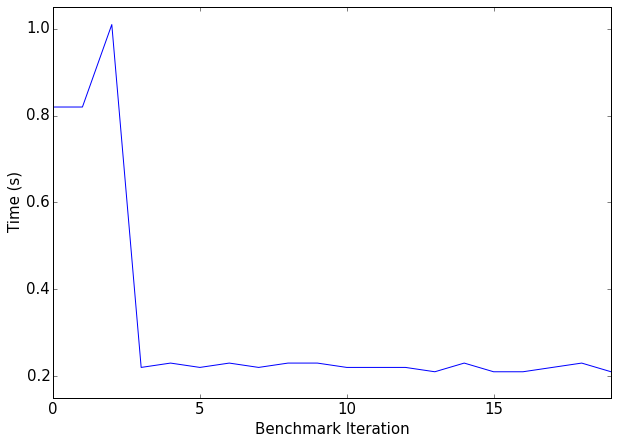
\includegraphics[width=.4\textwidth]{img/trad}
\caption{\laurie{the problem here is that we say `fictional', but the data looks vaguely real. we'd do better to make an obviously-not-real data figure, so that users can't misinterpret it. the glowworm proposal has something along these lines in it already} This (fictional) chart illustrates the commonly accepted understanding
of JIT performance. Early iterations of a benchmark perform poorly during the
warmup phase of the JIT. Once the JIT begins emitting native code (around
iteration 3) the latency of the benchmark is consistently small, with a small
amount of variation due to the operating system and execution environment.}
\label{fig:trad}
\end{figure}

The graph in Figure~\ref{fig:trad} demonstrates the impact that we might
expect JIT warmup to have upon a benchmark running repeatedly within a
single process. In the first iteration (iteration 0), the VM has no compiled
code for the benchmark and therefore it runs slowly in a profiling
interpreter. After two or three iterations the profiler has collected enough
information for the JIT the begin compiling. For this fictional VM,
compilation is more expensive than the profiling interpreter, thus it is
characterised by the spike at iteration 2. \footnote{The cost of
the profiling interpreter relative to that of compilation vary on a per-VM
basis.}At iteration 3, the JIT has compiled all of the code necessary to
efficiently run the benchmark. Subsequent iterations use the compiled code
and therefore run with improved performance. In other words, peak
performance is achieved at iteration 3. Note however that the measured times
for iterations $\geq 3$ are not quite the same. This is because there are many
sources of random variation that impact benchmark measurements. Random
variation can be introduced by the underlying operating system (e.g. by
context switches), or by the VM itself (e.g. garbage collection).  Generally
speaking, we expect peak performance measurements to be fast and ``mostly
constant'', with only small random variations distributed around a constant
mean~\cite{XXX}.  Ideally it would be possible to identify and control the
sources of random variation, allowing us to measure only the performance
characteristics of the VM. In practice however, this is very difficult.

A handful of methodologies -- most notably
\cite{kalibera12quantifying,kalibera13rigorous} -- require experimenters to take
warmup into account when benchmarking. We therefore set out to quantify how long
it takes various JIT compiled VMs to warmup. However, it soon became apparent to
us that our understanding of warmup is extremely naive:


\section{Methodology}
\label{sec:methodology}

To compare the warmup behaviour of different VMs, we created a carefully
designed experiment. The basic idea is simple: we take a number of
micro-benchmarks derived from the Computer Language Benchmarks Game (CLBG) and
run them in a loop of 2000 iterations against a number of VMs. We then analyse
the resulting data for information about warmup. Our experiment is designed to
control as many potentially confounding variables as is practical.

In this section we detail the set of benchmarks we use; the VMs under
investigation; the \krun system we have developed to reliably run benchmarks;
and the hardware we used. Readers may wish to note that we use two terms defined
by \cite{kalibera13rigorous}: \emph{iterations} are in-process repetitions of a
process; \emph{executions} create a new process to run a benchmark in.


\subsection{The CLBG micro-benchmarks}

We used the \binarytrees, \richards, \spectralnorm, \nbody, \fasta, and
\fannkuch microkbenchmarks from the CLBG (taking the particular implementations
from those used in \cite{bolz14impact}), with implementations in Java,
Javascript, Python, and Ruby. Readers can be forgiven for initial scepticism
about this set of micro-benchmarks. They are small, deterministic, and widely
used by VM authors as optimisation targets. In general they are more effectively
optimised by VMs than arbitrary programs; when used as a proxy for other types
of programs (e.g.~large programs), they tend to overstate the effectiveness of
VM optimisations. In our context, this weakness is in fact a strength: we need
small, deterministic, and widely examined programs so that we can test
hypothesis \hypone. Looked at another way, if we were to run arbitrary programs
and find unusual warmup behaviour, a VM author might reasonably counter with
``you have found the one program that exhibits unusual warmup behaviour''.

Our first task was to ensure that our micro-benchmarks are deterministic at the
user's level. We define this as benchmarks taking precisely the same path
through the Control Flow Graph (CFG) on each execution and iteration. Note that
this definition of determinism a) can be checked by the user b) does not
preclude the VM having other types of non-determinism when executing a benchmark
(e.g.~objects in memory may be collected in a non-deterministic fashion). We
first instrumented each micro-benchmark with \texttt{print} statements at each
control flow point and ran them for \laurie{XXX} iterations. This showed that
the \fasta benchmark was non-deterministic, using a random seed which was
initialised only on the initial load of the program; thus each iteration of the
program returned different random numbers, causing different paths to be taken
through the CFG. We removed this non-determinism by putting the seed
initialisation in the main loop of the benchmark. Bearing in mind surprising
results such as the important of link order \cite{mytkowicz09surprising}, we
then recompiled all the VMs and ran them on a different machine to see if any
compile-time constants affected determinism. \laurie{this is still ongoing work}

We run benchmarks for 2000 iterations. We explicitly do not force a garbage
collection after each iteration, as a VMs GC is an important factor in warmup.
\laurie{how many executions?}


\subsection{VMs under investigation}

\laurie{i thought we were also including C versions of the benchmarks?}

We ran the benchmarks on a collection of modern programming language VMs:
\begin{description*}
\item[PyPy-2.6.0] A meta-tracing VM for Python-2.7.
\item[Java8-b132] Oracle's Hotspot VM for Java.
\item[Graal-dev~\footnote{Graal version 9dafd1dc5ff9.}] Oracle's next-gen
Java VM.
\item[LuaJIT-2.0.4] A tracing JIT for Lua.
\item[HHVM] Facebook's PHP JIT.
\item[JRuby/Truffle-dev~\footnote{JRuby/Truffle version 7b4cee81891f.}] A
Ruby VM using Graal/Truffle.
\item[V8-4.5.38] Google's JIT for Javascript.
\item[CPython-2.7.10] The reference Python implementation.
\end{description*}

All bar one of
these VMs include a JIT compiler. CPython is a simple interpreter written in C,
that was included as a kind of sanity check (it should not exhibit JIT warmup
characteristics).


\subsection{\krun}

Running benchmarks is a conceptually easy task that has many fiddly details in
practise: VMs need to be compiled; benchmarks need to be run in a consistent
environment; and errors need to be detected and reported to the user. We created
the \krun system to enable us to reliably run and rerun benchmarks on different
machines. In essence, \krun takes in a configuration file which enables it to
automate what are traditionally manual and error-prone tasks. Benchmarks are
written to output iteration timings to \texttt{stdout} which \krun then collects
into a single output.

Some of the factors that \krun controls are platform-specific, and we detail
those in subsequent subsections. However some aspects are common to all
platforms. Most notably, \krun does its best to prevent machines from
overheating, which tends to lead to CPUs being throttled (and thus distorting
performance results). Temperature readings are taken when \krun starts; after
each execution, \krun waits for the CPU to cool to within 10\%{} of this initial
reading. If the system fails to cool down, \krun terminates. \laurie{is there a minimum sleep period?}

Other useful common features include the following. \krun specifies a consistent maximum heap
\texttt{ulimit} for each VM (2GiB). It also monitors \texttt{dmesg} output,
emailing the user when possibly important output appears in it (filtering out
some unimportant information on a platform-specific basis, to avoid overwhelming
the user). \laurie{Is it fair to say something like ``This is surprisingly
informative: we removed one benchmarking machine form our suite when
\texttt{dmesg} output showed that it was occasionally overheating, leading to
the CPU being throttled''?}


\subsection{Machines used}

We used four machines and two operating systems:
\begin{description*}
  \item[\bencherthree] A quad-core i7-4790K 4GHz machine running Debian 8. Turbo boost
    and hyper-threading were disabled in the BIOS.
  \item[\bencherfive] A quad-core i7-4790 3.6GHz machine running Debian 8. Turbo
    boost and hyper-threading were disabled in the BIOS.
  \item[\benchersix] Identical hardware to \bencherfive, but running OpenBSD 5.7. Turbo
    boost and hyper-threading were disabled in the BIOS.
  \item[\bencherseven] The ARM machine. \laurie{more details needed}
\end{description*}

On Intel machines, we disable turbo boost and hyper-threading. Turbo boost is a
feature which allows CPUs to temporarily run in an extremely high-performance
mode; this eventually causes the CPU to exceed its safe thermal limit, and is
thus a temporary effect. Turbo boost can thus cause long-running processes to
appear to suddenly slow down. Hyper-threading gives the illusion that a single
physical core is in fact more than one core. Different programs running in
hyper-threads can thus interfere with each other in complex ways.
Hyper-threading is thus a source of noise, but has no benefit to our benchmarks,
where we do not even make use all of the cores in such machines.


\subsubsection{Linux}

On Linux, \krun controls several additional factors.

First, it attempts to fix the CPU frequency to the highest
possible `recommended' value (i.e.~below the overclocking range). This is achieved by disabling Intel
p-states support in the kernel and setting the CPU governor to \texttt{performance}
mode.~\footnote{This is our best attempt at obtaining a constant CPU clock
speed. The Linux kernel documentation states that ``the idea that frequency can
be set to a single frequency is fiction for Intel Core
processors''~\cite{XXX}.}

Second, it runs benchmarks on a single CPU core, reducing the cost of processes
being forcibly moved to different cores. This is achieved through Linux's
\texttt{isolcpus} feature. \laurie{this sentence scares me. i thought it would
mean that kernel threads wouldn't run on the core!} This means that benchmarks
share a CPU only with kernel threads. In theory a core can be fully isolated,
however the Linux tool to enable this is currently broken
\url{https://bugs.debian.org/cgi-bin/bugreport.cgi?bug=796893}.

Third, \krun minimises the effects of the Linux kernel profiler \laurie{can we
be clearer about what this thing is actually doing?}. We found this to introduce
substantial noise into benchmarks, since it dynamically adjusts (lowers
\laurie{can it only ever lower? can it raise?}) its sample rate if it is found
to spend too much CPU time. While this feature cannot be entirely disabled on
x86-64, \krun reduces its frequency to once per second, minimising noise.


\subsubsection{OpenBSD}

\laurie{sysctl to 100 and \texttt{apm -H} but p-states...?}


\subsection{Other stuff}

\edd{data layout (e.g. ASLR, don't re-run in separate sessions)}
\edd{quartile regression}


\section{Results}
\label{sec:Results}

After running all benchmarks as described we analysed the benchmarks in a
two-step process. In the first step we visually inspected the run sequence
graphs of all the benchmark executions, per benchmark and virtual machine. In
doing so we noted whether the virtual machine followed the expected warmup
behaviour for this benchmark as described in Section~\ref{sec:warmup}. This was
the case of \cfbolz{add numbers} X out of Y benchmarks. In a second step we
identified groups of ``anomalies'', i.e. repeating ways of how benchmark
executions deviated from the expected warmup behaviour. In the following we will
present the run-sequence diagrams of benchmarks that have expected warmup
behaviour, as well descriptions and examples for all the anomalies.

\cfbolz{need some examples of nice benchs}
\cfbolz{we need a table which does all the categorizations, and examples}

\cfbolz{observations 2x2: widely varying performance on the same machine, late
phase change not always there, another case: bimodality, slowdowns are
sometimes speedups, different repeating shapes across machines}

\cfbolz{safety checks: are outliers deterministic across different processes?
is the behaviour generally the same looking? do some checks on other OS,
machine architecture, frequency scaling independent}


\sarah{Warm-up takes longer than expected, by comparison with the idealised JIT
described in Section 2.}


\subsection{Outliers}
\label{sub:outliers}

Outliers are iterations of a benchmark that take significantly longer than the
other iterations, even taking the randomness of the benchmark iterations into
account.

Figure~\ref{fig:examples:outliers1} shows one such example, which includes an
outlier around iteration $900$ that runs more than $0.5s$ slower than the
measurements either side of it.

\begin{figure}[h!]
\centering
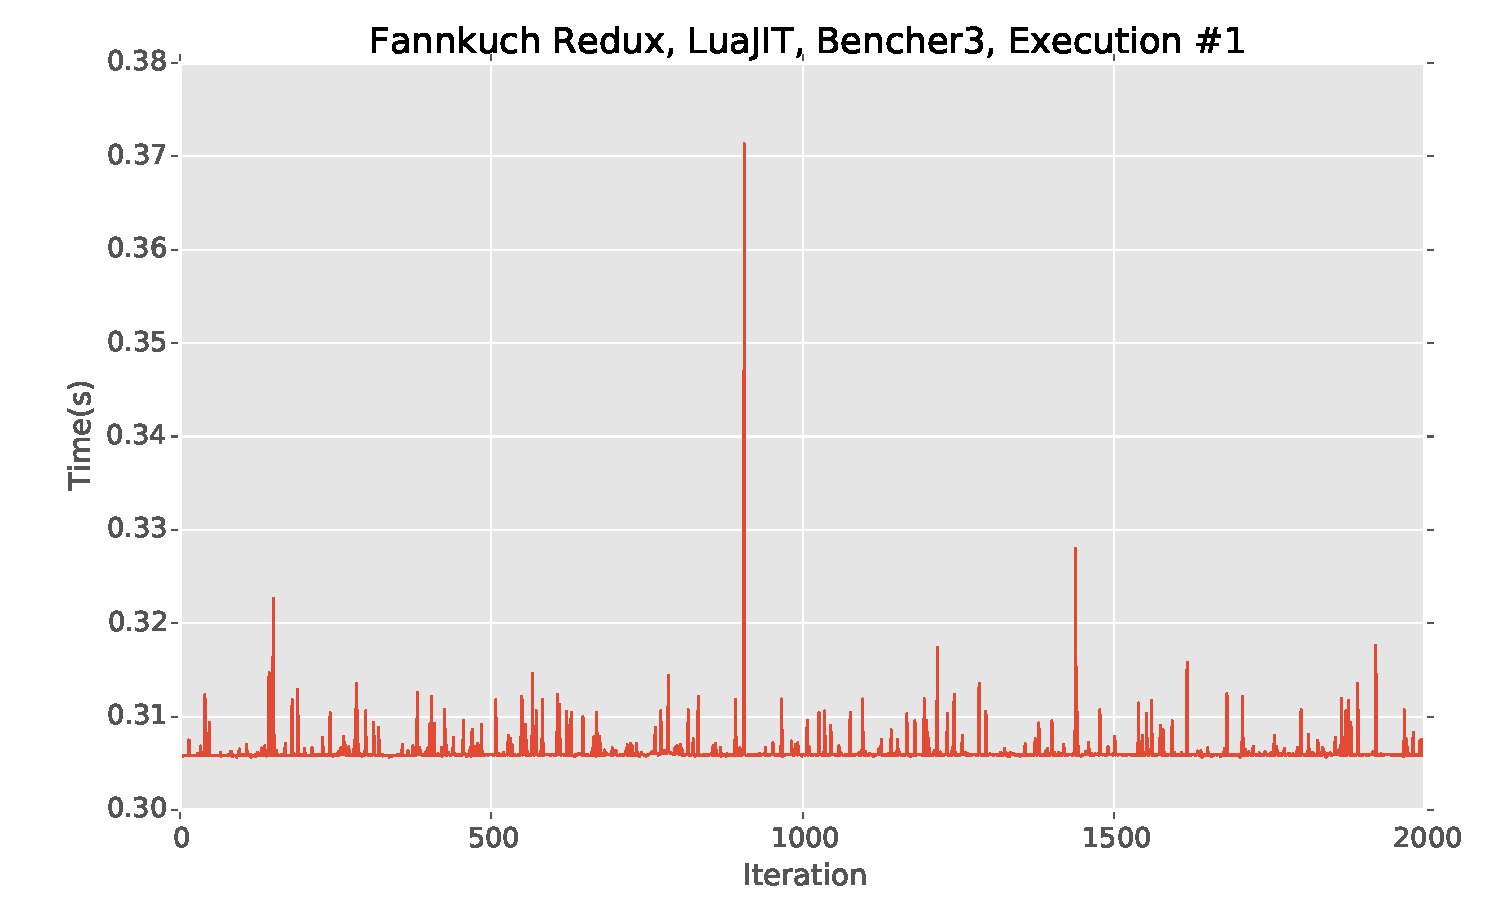
\includegraphics[width=.46\textwidth]{examples/outliers1}
\caption{Example of a benchmark with outliers.}
\label{fig:examples:outliers1}
\end{figure}


\subsection{Slowdowns}
\label{sub:slowdowns}

\sarah{This is one area were the sliding-window average might be useful (i.e. in detecting a slow-down).
One possible way forward would be to find a technique for performing hypothesis testing on time-series data, then running tests to determine whether the sliding-mean in one part of the chart is significantly different to the sliding-mean in an earlier phase of the execution.
This technique would also help to determine precisely when the warm-up phase is over and the JIT has kicked in.}

A few benchmarks exhibit slow downs, where the first few iterations of a
benchmarks are faster than the eventual mean after ``warm up''.

Figure~\ref{fig:examples:slowdown1} shows one such example.

\begin{figure}[h!]
\centering
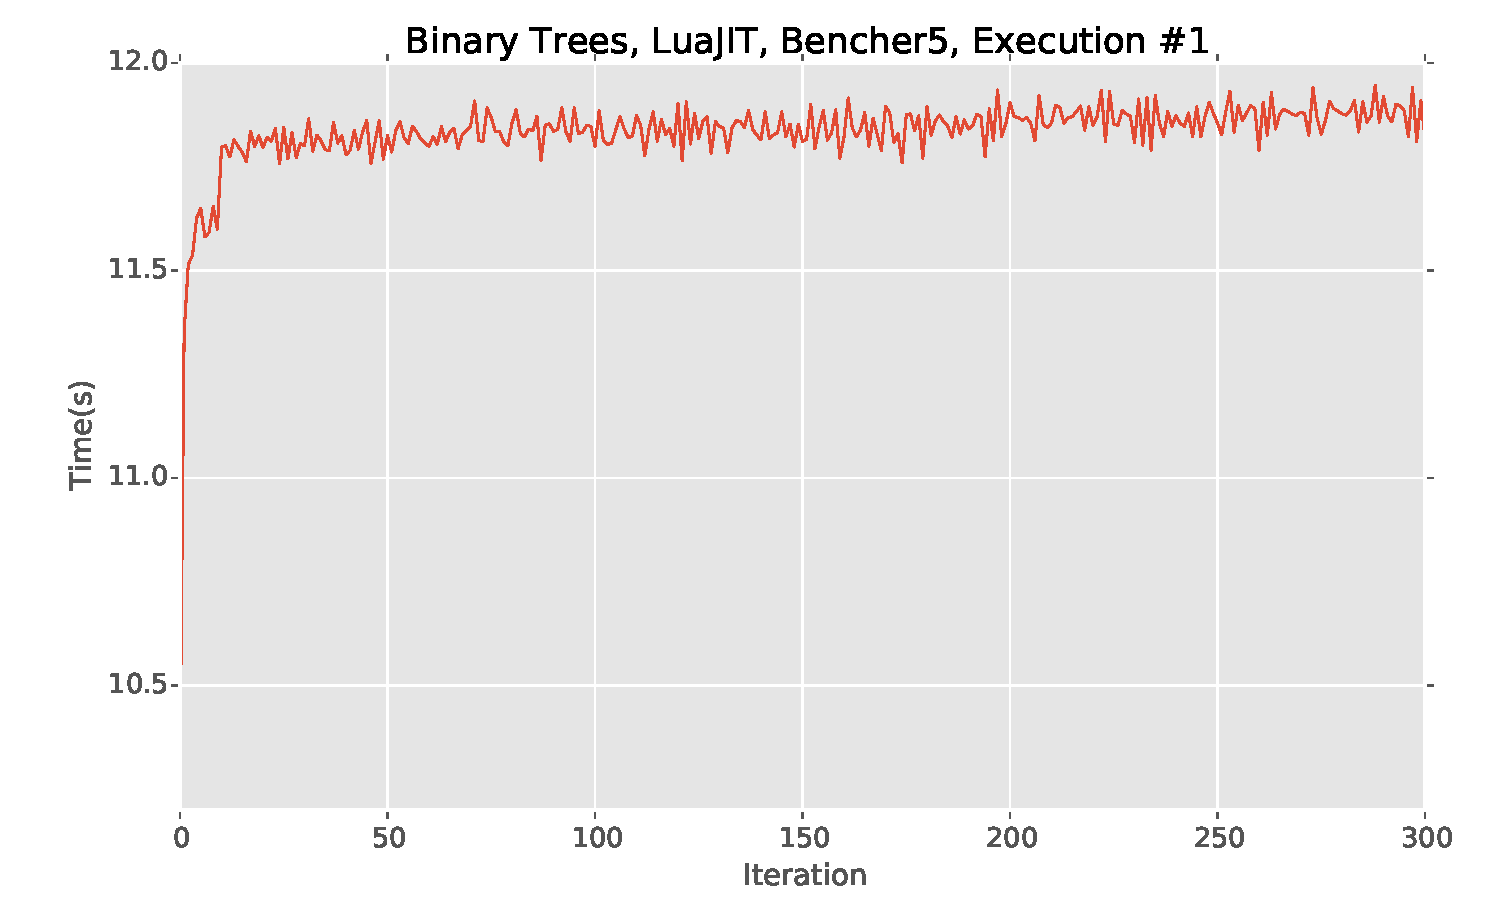
\includegraphics[width=.46\textwidth]{examples/slowdown1}
\caption{Example of a benchmark with a slowdown.}
\label{fig:examples:slowdown1}
\end{figure}



\subsection{Cyclic Behaviour}
\label{sub:cyclic}

Cyclic behaviour occurs in a number of benchmarks, which is a pattern of $n$
iterations that have similar timing results and keeps repeating across the
benchmark runs.

Figure~\ref{fig:examples:cycles1} shows one such example.

\begin{figure}[h!]
\centering
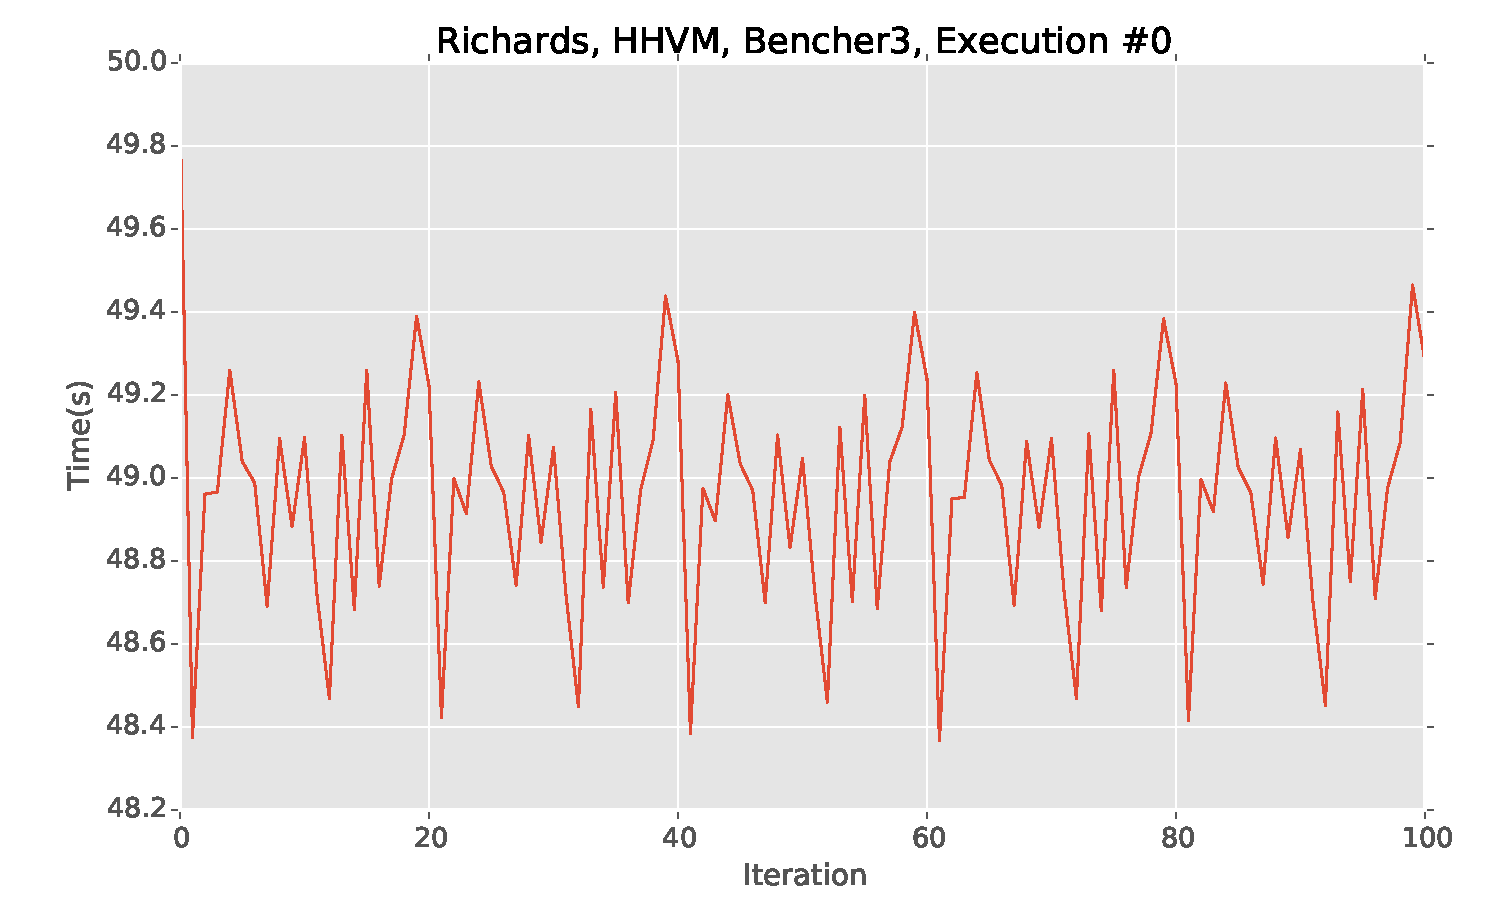
\includegraphics[width=.46\textwidth]{examples/cycles1}
\caption{Example of a benchmark with cycles.}
\label{fig:examples:cycles1}
\end{figure}


\subsection{Late Phase Changes}
\label{sub:phase}

Late phase changes occur in benchmarks where after many iterations the benchmark
changes behaviour, either by getting slower or faster, or by producing a
different pattern of randomness.

Figure~\ref{fig:examples:late1} shows one such example.

\begin{figure}[h!]
\centering
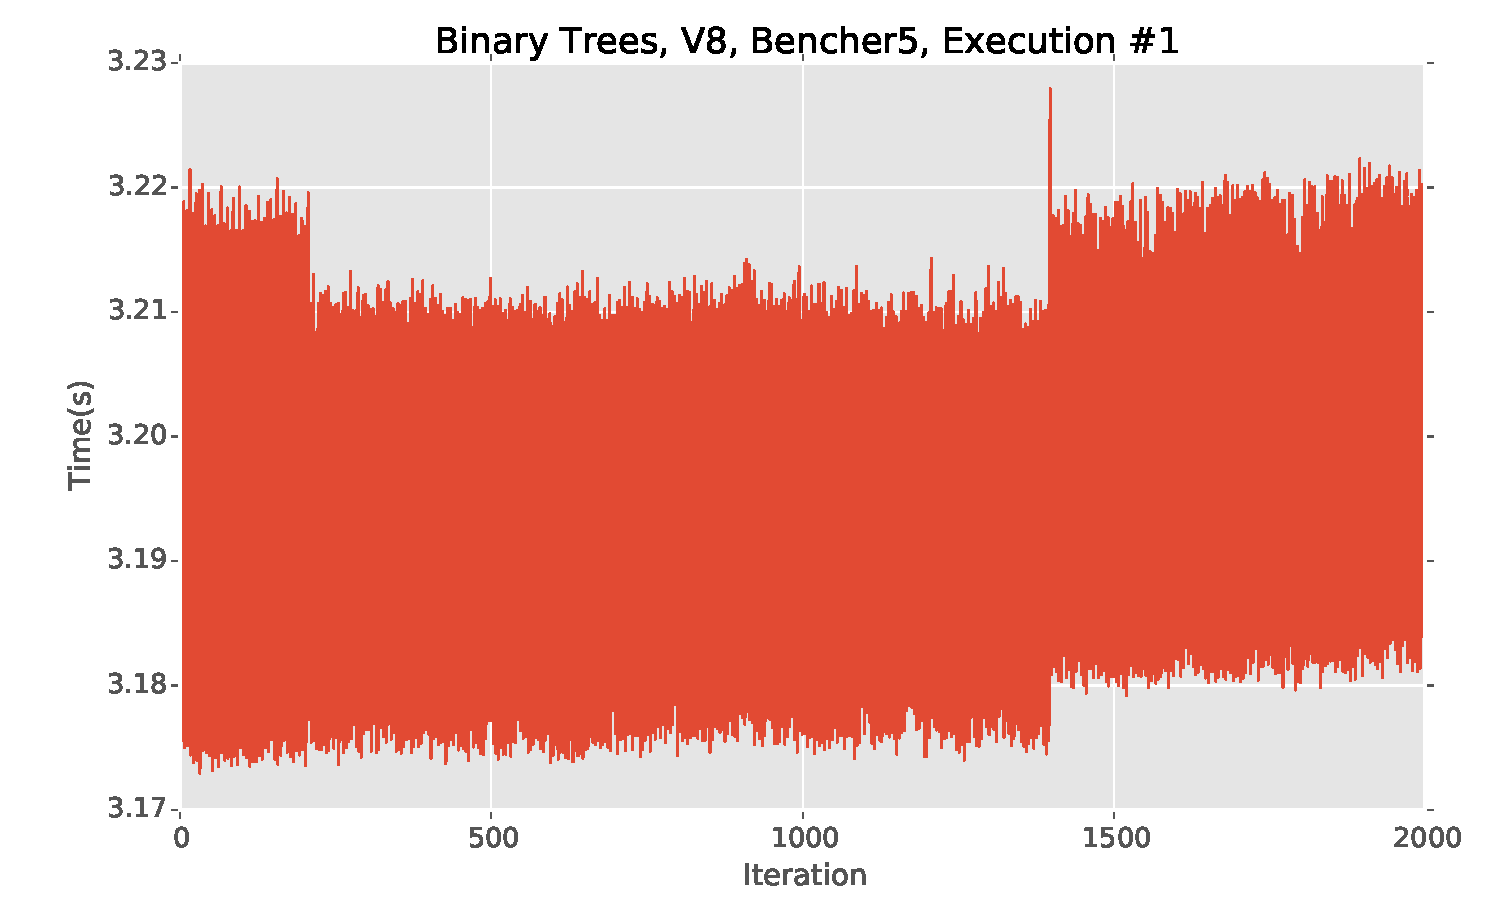
\includegraphics[width=.46\textwidth]{examples/late1}
\caption{Example of a benchmark with late phase changes.}
\label{fig:examples:late1}
\end{figure}

\subsection{Inconsistent Effects}
\label{sub:inconsistent}

\edd{Many of the effects we saw are consistently weird. Some are not. What
do we think of this as a section?}
\sarah{Sounds good, what about a section on unexpectedly long warmup?}

Figure~\ref{fig:examples:consistent_weirdness1} shows a case where
unexpected behaviours are consistent between machines and executions.
Figure~\label{fig:examples:inconsistent_weirdness1} shows an example where
effects differ between both machines and executions.

\begin{figure*}[h!]
\centering
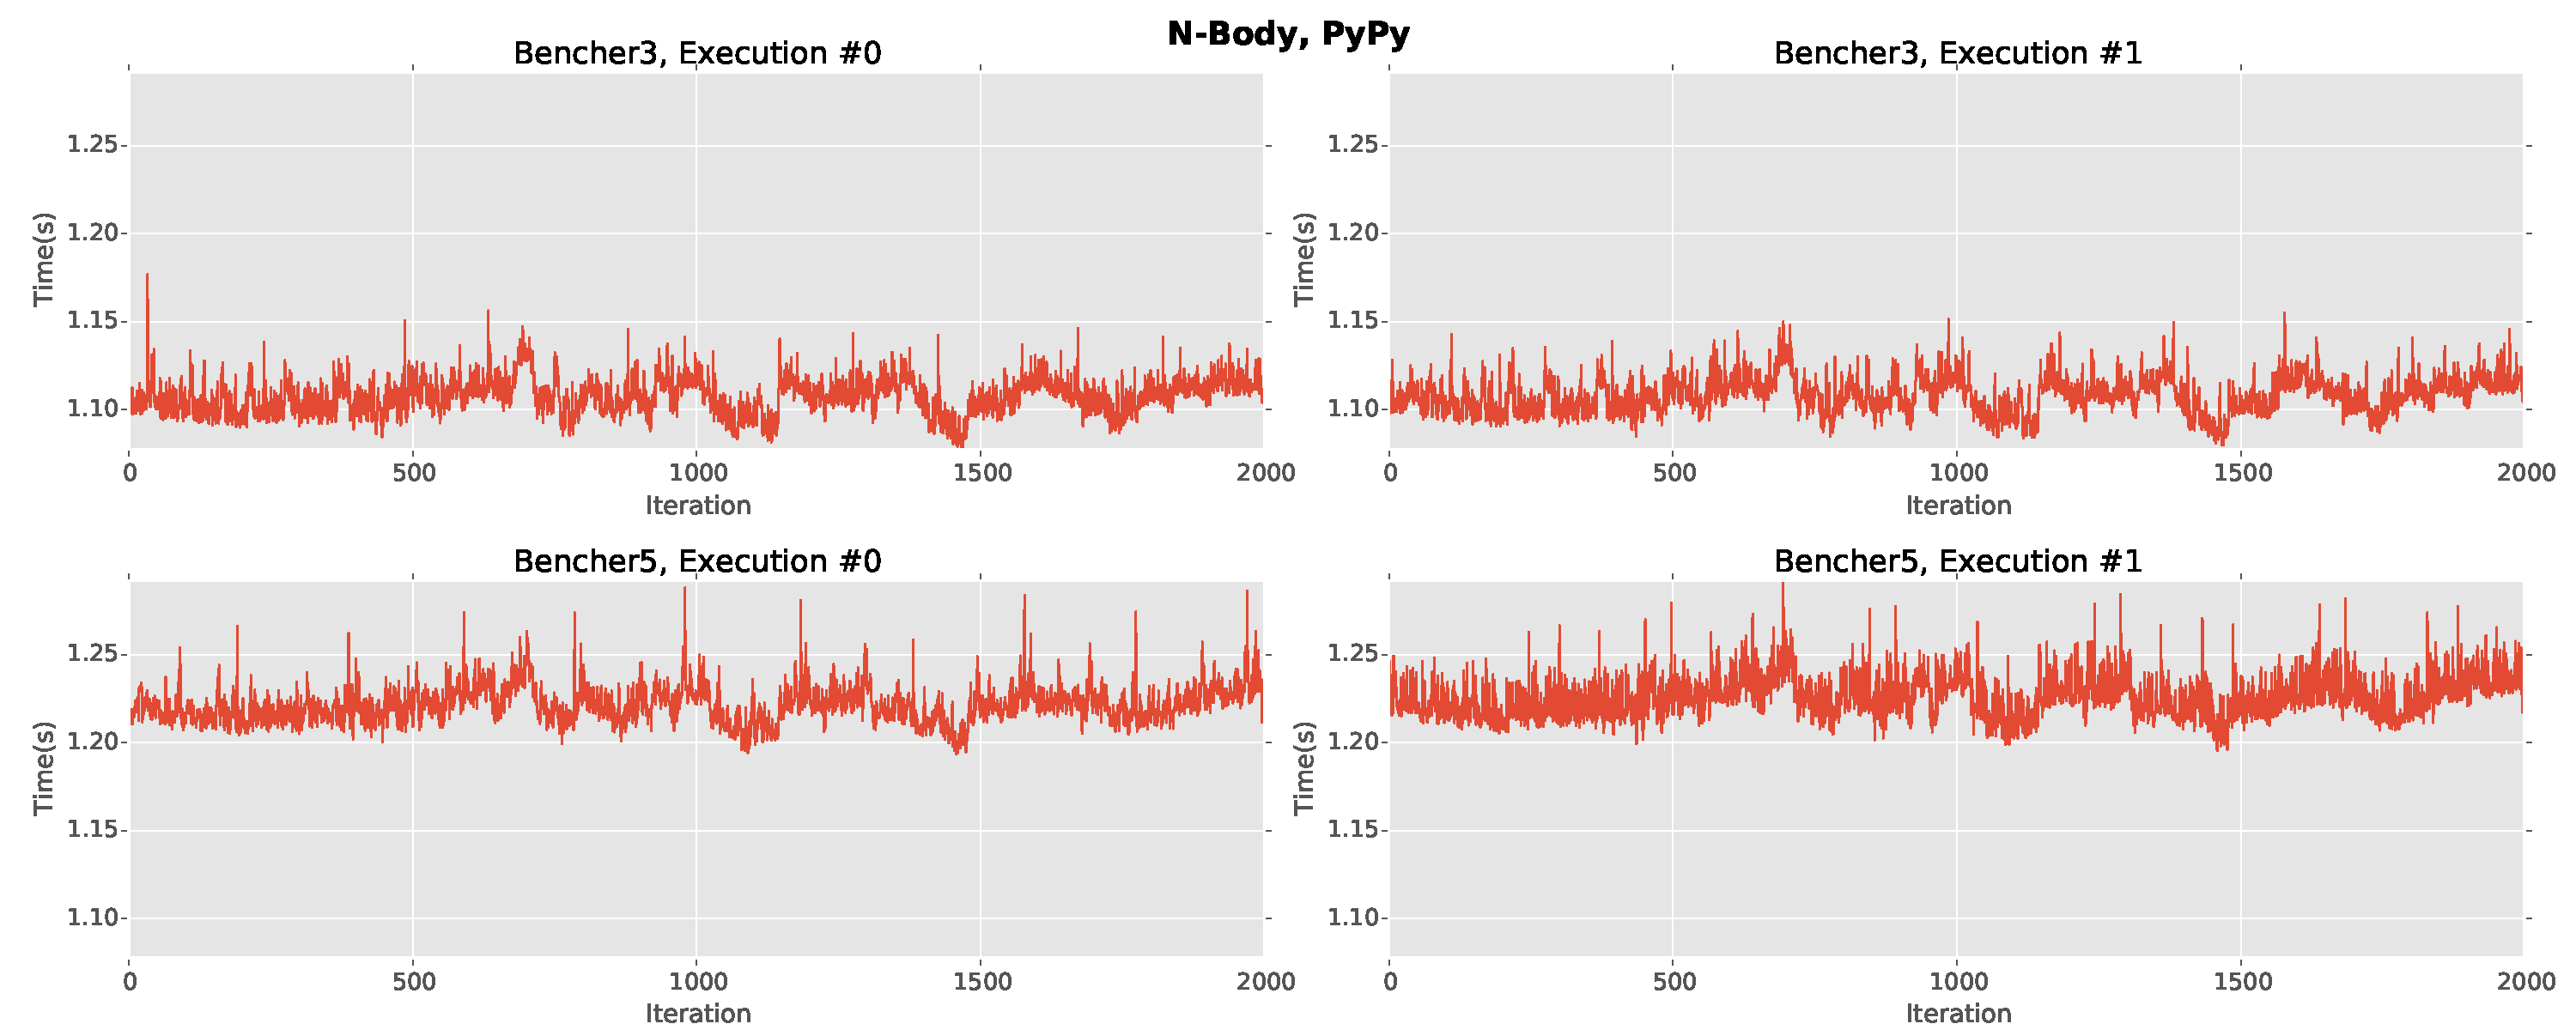
\includegraphics[width=\textwidth]{examples/consistent_weirdness1}
\caption{Example of a benchmark whose effects are consistent between machines and executions.}
\label{fig:examples:consistent_weirdness1}
\end{figure*}

\begin{figure*}[h!]
\centering
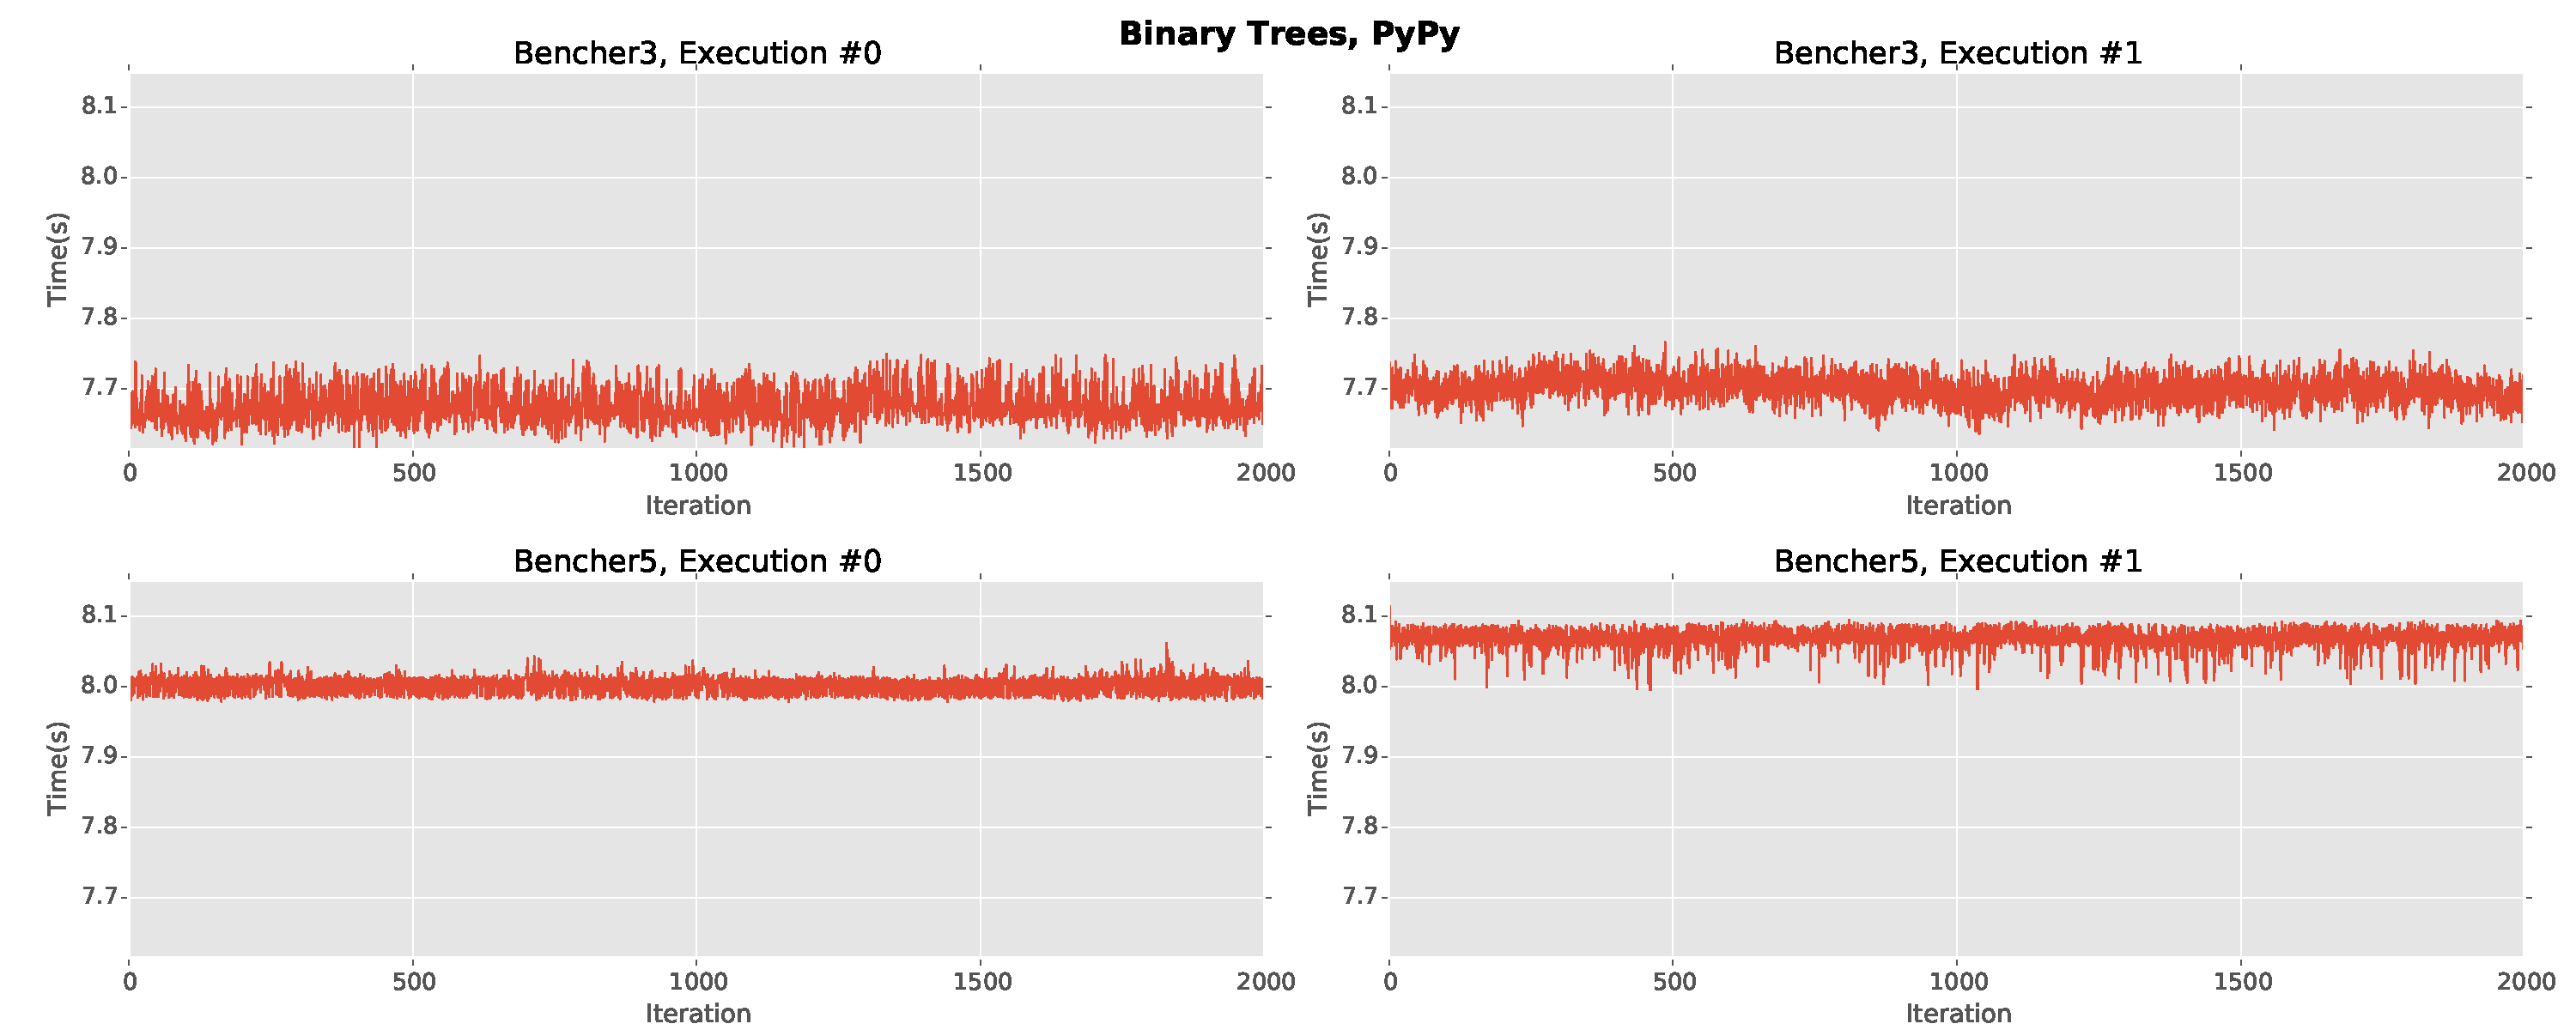
\includegraphics[width=\textwidth]{examples/inconsistent_weirdness1}
\caption{Example of a benchmark whose effects are inconsistent between machines and executions.}
\label{fig:examples:inconsistent_weirdness1}
\end{figure*}


\section{Threats to Validity}
\label{sec:threats}

While we have designed our experiment as carefully as possible, we do not
pretend to have controlled every possibly confounding variable. For example,
because of the large quantity of software we had to install, and because we used
different operating systems, we can not guarantee that the VMs were compiled in
the same way on each machine. \laurie{if we're lucky, our cross-machine results
will be fairly stable, which will allow us to say something like ``despite the
possible variation across our machines, we got fairly stable results, suggesting
that this was not a significant issue in practise''.}

\sarah{threats to validity: there may be some confounding variables that have
not been controlled in these experiments. There may be bugs in the JITs that
are being measured.  The benchmarks in the guest languages might be similar
enough that some important classes of behaviour have been missed, because the
benchmarks here do not trigger those behaviours.  There may be some un-thought
of explanation for weird JIT behaviour which has nothing to do with the JIT.}


\section{Discussion}
\label{sec:Discussion}

  - discussion:
    - need to give up naive definition of warmup
    - unrealistic to get rid of these anomalies
    - some of benchmarking wisdom is wrong in the presence of this stuff
\sarah{Need some way to model the behaviour of JITs and perform hypothesis tests (so that people can answer questions like 'does this change in the VM actually make the JIT faster?').}

\section{Conclusions}
\label{sec:conclusion}

\bibliographystyle{abbrvnat}
\bibliography{bib}


\end{document}

